\chapter{Experiments}
\label{c:experiments}
\IMRADlabel{results}



In this chapter we will present all environments we experimented with as well as \emph{Hyper-Experiments}, \ac{ie} experiments with the hyperparameters and their influence on the algorithm performance (in terms of the prediction error and similar metrics, not the computing time).

\section{Environments and Experiment Setup}
	We will not introduce to you the environments and the setup for each environment that we used. We will not discuss any results here,see~\autoref{c:discussion} for that. Do generate the data, you have to run the file \texttt{src/data.py} with the desired experiment ID as the first argument, \ac{eg} \texttt{python src/data.py pendulum\_damped}. If no argument is given, a regeneration of the data from all experiments is triggered. For each of the following environments we summarize the most important data about the environment at the start of the subsection, including the experiment ID.

	\subsection{Proof of Concept: Classic LGDS}
		\begin{itemize}
			\item Experiment ID: \texttt{lgds}
		\end{itemize}

		As a proof of concept and to empirically verify our proof on the exactness of the cubature rule and hence the similar expected performance for plain linear systems, we benchmark our algorithm against a simple linear system. The linear system has a two-dimensional state \( \vec{s} \coloneqq (x_2, x_2)^T \) with the dynamics
		\begin{equation*}
			\dot{\vec{s}} =
				\begin{bmatrix}
					 0 & 1 \\
					-1 & 0
				\end{bmatrix} \vec{s}
		\end{equation*}
		The initial state \( \vec{s}_1 \) is sampled from a Gaussian with mean \( (0.1,\, 0.2)^T \) and covariance \( \diag\big(10^{-5}, 10^{-5}\big) \). The system is integrated using the implicit Runge-Kutta Radau~IIA~\cite{guglielmiImplementingRadauIIA2001} method with an evaluation interval of \( h = 0.1 \) for \(T 0 240\) time steps where only the first \(T_\train = 120\) steps are used for training and the remaining \(120\) are used for validation. In total \(N = 3\) sequences are generated, each with a different initial value. The raw data is shown in~\autoref{fig:envLgds}.

		\begin{figure}
			\centering
			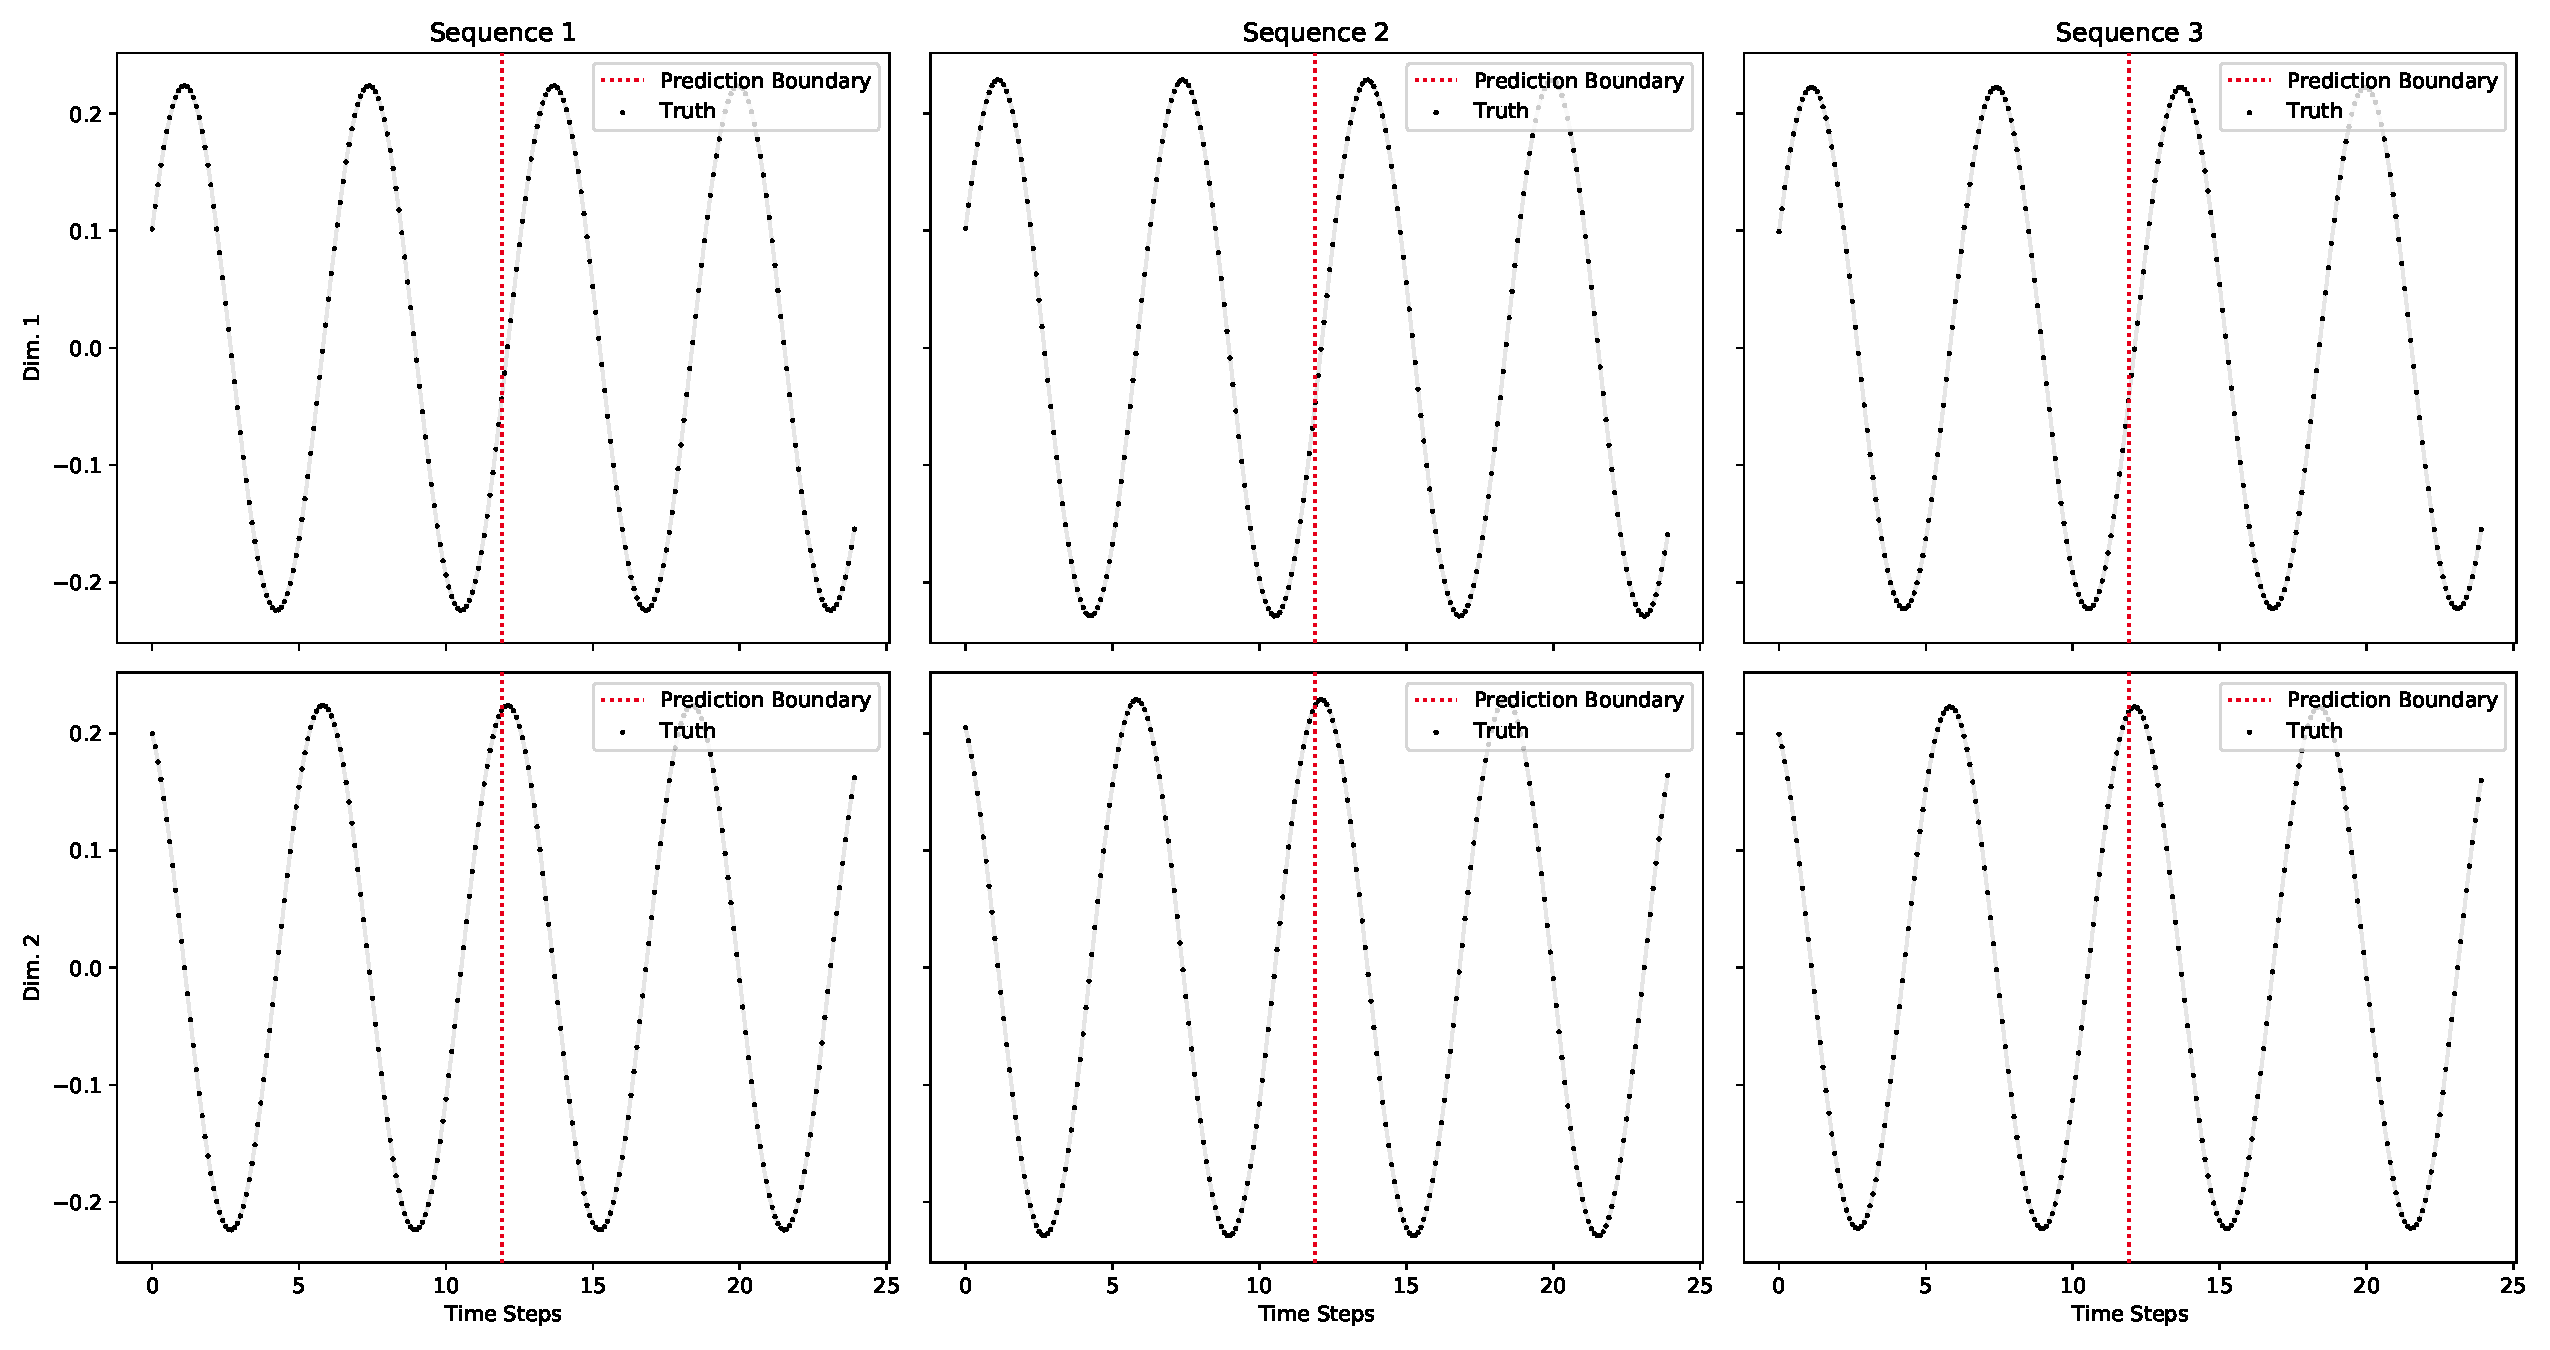
\includegraphics[width=\linewidth]{figures/experiments/environments/observations-lgds.pdf}
			\caption{Plot of the raw data used for training the proof-of-concept \ac{lgds} environment. The black dots represent the actual data points, all before the red "prediction border" are used for training, the rest for validation. The faint gray line emphasizes the connection between the data points and that they are actually generated from a dynamical system.}
			\label{fig:envLgds}
		\end{figure}
	% end

	\subsection{(Damped) Pendulum}
		\todo{Exp Envs: (Damped) Pendulum}
	% end

	\subsection{Gym Pendulum}
		\todo{Exp Envs: Gym Pendulum}
	% end

	\subsection{Gym Cartpole}
		\todo{Exp Envs: Gym Cartpole}
	% end

	\subsection{Gym Acrobot (Double Pendulum)}
		\todo{Exp Envs: Gym Acrobot}
	% end
% end

\section{Experiments with Hyperparameters}
	% Probably more if I can run more experiments… But all other hyperparameters are not as interesting.

	\todo{Exp: Hyper-experiments}

	\subsection{Influence of the Latent Dimensionality}
		\label{subsec:experimentLatentDim}

		\todo{Exp Hyper: Latent Dim}
	% end
% end
